\chapter{Surface Flow -- H-Processes}
\label{sec:Surface}
%
This chapter deals with surface flow. Surface flow or overland flow is a thin sheet of water flow which occurs when soil is infiltrated to full capacity and excess water, from rain, snowmelt, or other sources flows over the land. Generally, it causes a gathering of the runoff into discrete stream channels. The governing equations are introduced in Sec.~\ref{sec:SurfaceTheory} and the benchmarks in Sec.~\ref{sec:SurfaceBechmarks}. Surface flow is solved one- and two-dimensionally in the benchmark examples.
%
\section{Theory}
\label{sec:SurfaceTheory}
%
Overland flow can be described by the diffusive and kinematic wave approximations of the Saint-Venant equations. The diffusive wave equation \cite{Therrien:04} is given by 
\begin{eqnarray}
\phi_a\frac{\partial H_a}{\partial t} + \bar\nabla\cdot \left( H \mathbf q \right) = q_s
\label{eqn:OLF_Governing}
\end{eqnarray}
%
where surface water depth $H_a$ is used as a primary variable in the overland flow calculation, $H$ is the mobile water depth, $\bar\nabla$ is two-dimensional Nabla-Operator and $q_s$ is the source/sink term. $0 \leq \phi_a(H_a) \leq 1$ is the surface porosity which is unity for flow over a flat plane and varies between zero and unity for flow over an uneven surface. Surface roughness is parameterized with the immobile water depth $a$ such that the surface water depth is given by  $H_a = H + a$ (see Fig.~\ref{OLF:SurfaceFlow}).

Empirical resistance to flow relationships leads to \cite{VKwaak:99}
%
\begin{figure} [htb!]
 \centering
 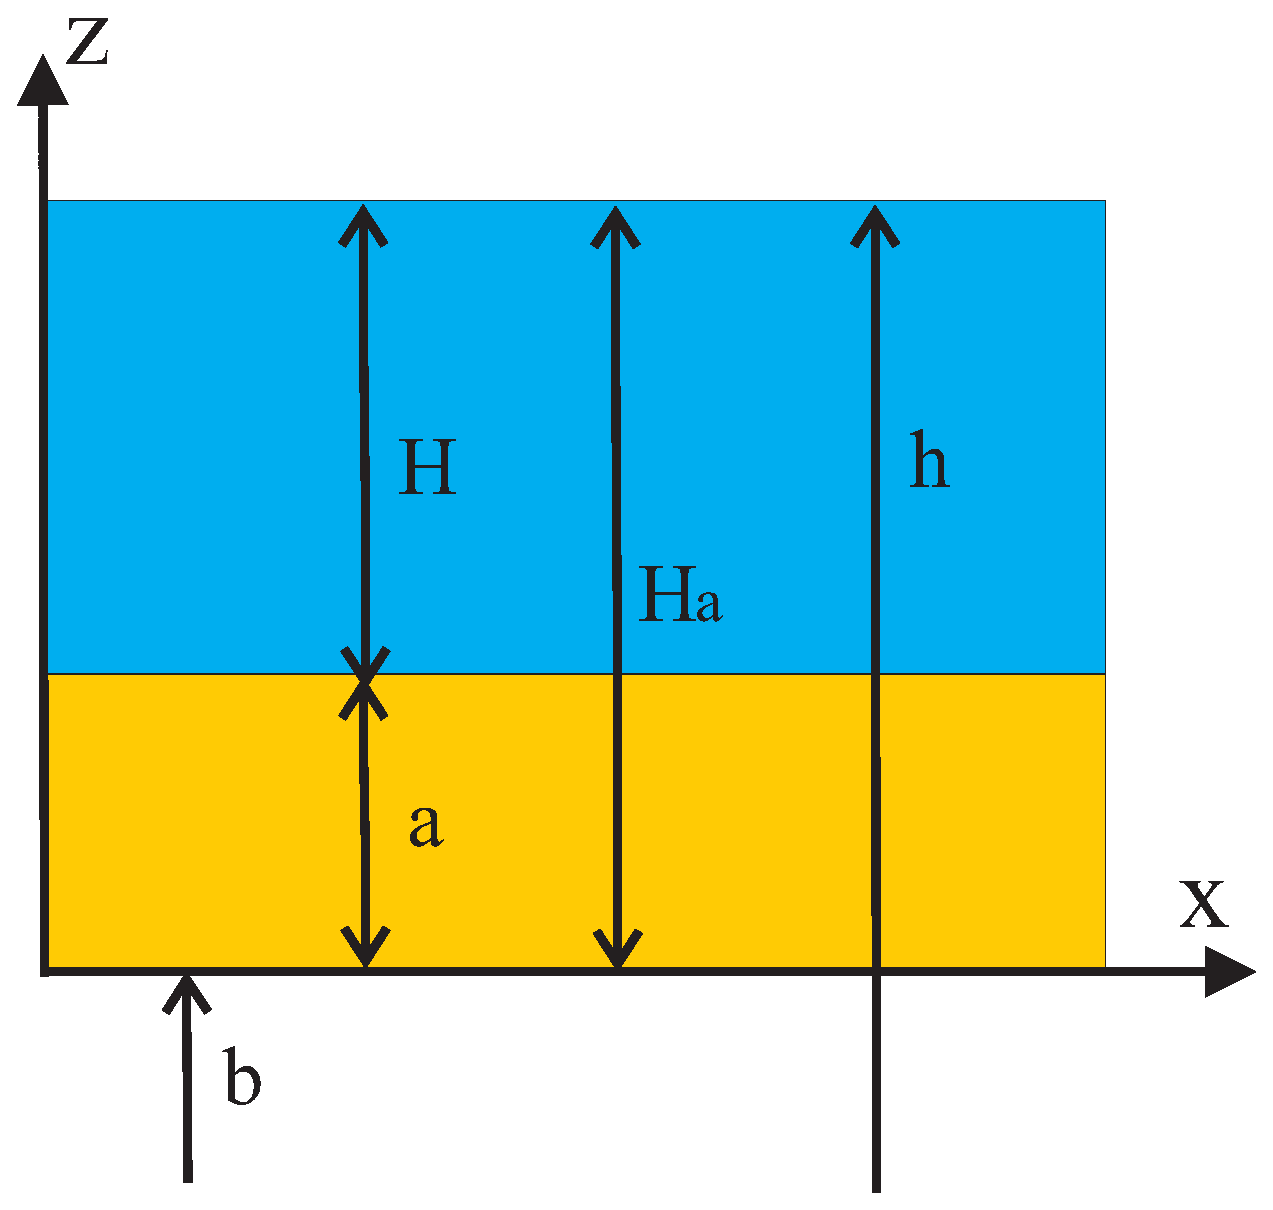
\includegraphics[width=0.75\columnwidth] {H_SFC/figures/SFlow.eps}
 \caption{The diagram for the relationships of surface water depth, mobile/imobile water depth and surface water head}
 \label{OLF:SurfaceFlow}
\end{figure}
%
\begin{eqnarray}
\mathbf q = -\frac{C R^l}{S_s^{1-j}} \bar\nabla h 
\label{eqn:fluxOverland}
\end{eqnarray}
%
where%
\begin{eqnarray}
S_s =\left[
\left(\frac{\partial h}{\partial x}\right)^2  +
\left(\frac{\partial h}{\partial y}\right)^2
\right]^{1/2} 
\label{eqn:OLF_Ss}
\end{eqnarray}
%
where $h$ is the surface water head and given by $h = H_a + b$ where $b$ is the bottom elevation. For overland flow, the resistance to flow relationship considers only the bottom friction such that the hydraulic radius is given by $R=H$. 

The surface bottom friction parameters $C$, $j$, $l$ are evaluated from the Darcy-Weisbach relationship. The turbulent Ch\'ezy relationship is obtained with $j = l = 1 / 2$ and $C = C_t$ is the Ch\'ezy coefficient. Correapondingly, $j = 1$, $l = 2$ can lead to the laminar Ch\'ezy relationship. $j = 1/2$, $l= 2/3$ and $C= 1/n$ can lead to the Manning relationship, where $n$ is Manning coefficient.

For one-dimensional description of rivers, Eq.~\ref{eqn:fluxOverland} becomes \cite{Jul:02}
%
\begin{eqnarray}
\mathbf q = -\frac{C R^l}{|\partial h / \partial x|^{1-j}} \frac{\partial h}{\partial x} \label{eqn:fluxRiver}
\end{eqnarray}
%
where the hydraulic radius $R$ is determined by the flow cross-section $A_F$ and the wetted perimeter $P$, i.e. $R=A_F/P$.

For overland flow, the source/sink term is given by $q_s = q_p - q_d$, where $q_p$ is the precipitation rate, and outflow at the lower boundary $q_d$ is determined by normal depth, or critical depth.
%
\begin{eqnarray}
q_d^{norm}&=& CS_o^j H^l \\
q_d^{crit} &=& \sqrt{ gH^3}
\end{eqnarray}
%
The infiltration source-terms can be calculated with the Green-Ampt model.
%
\begin{eqnarray}
q_d^{GA} &=& K \left( \frac{H - \Psi}{\tilde{a}} \right) 
\label{eqn:OLF_Green_Ampt}
\end{eqnarray}
%
where $K$ is the effective hydraulic conductivity, $\Psi$ is the effective capillary drive, and $\tilde{a}$ is the location of the wedding front.
%
%
%-------BENCHMARKS--------------------------------------------------------------------------------------------------------------
%
%
\section{Benchmarking examples}
\label{sec:SurfaceBechmarks}
%
\subsection{One-dimensional precipitation runoff}
\label{sec:Govindaraju}
%
\subsubsection*{Problem definition}
%
These examples are based on the study by \cite{Gov:88} which compared solutions given by the Saint-Venant equations and its diffusive wave and kinematic wave approximations. The simulation parameters are given by \cite{Therrien:04}.
Constant precipitation is applied for $4 min$ to an initially dry plane with a lenght of $100m$ and a slope of $0.01$. The flow is assumed to continue uniformly at the lower domain boundary.
%
\subsubsection*{Initial and boundary conditions}
%
The initial water depth is $1\cdot 10^{-4}m$. The precipitation value is $4 \cdot 10^{-3} m/s$.
A normal depth boundary condition is assigned to the outlet and no-flow to the remaining boundary.
%
\subsubsection*{Material properties}
%
The time step size is $1 s$.
The domain is discretized with line or quadrilateral elements.
The line elements have a length of approximately $1m$ thoughout and the quadrangles $1m\times 1m$
For bottom friction Manning's relationship is used.
Simulation parameters and fluid characterstics are given in Tab.~\ref{OLF:govindarajuSetting}.
%
\begin{table}[H]
 \centering
 \caption{Parameters and fluid characteristics for one-dimensional precipitation runoff examples}
 \centering \label{OLF:govindarajuSetting}
 \begin{tabular}{llll}
 \hline\hline\noalign{\smallskip}
 {\bf Parameter} & {\bf Symbol} & {\bf Setting} & {\bf Unit} \\ \hline
 Manning coefficient & $n$  & $5.48\times 10^{-2}$ & $s/m^{1/3}$\\
 Immobile depth & $a$ & $0$ & $m$ \\
\noalign{\smallskip}\hline\hline
 \end{tabular}
\end{table}
%
\subsubsection*{Results}
%
A comparison of GeoSys with Hydrosphere and MODFLOW-Surface as well as solutions with the Saint-Venant and kinematic wave equations are shown in Fig.~\ref{OLF:govin_outlet}
%
\begin{figure} [htb!]
 \centering
 \includegraphics[width=0.75\columnwidth] {H_SFC/figures/govin.eps}
 \caption{Results for one-dimensional precipitation runoff examples}
 \label{OLF:govin_outlet}
\end{figure}
%
\subsubsection*{Benchmark deposit}
%
\begin{tabular}{|l|l|l|}
  \hline
  Benchmark & Problem type & Path in benchmark deposit \\
  \hline
  \emph{govin\_line} & H & benchmarks\verb \OVERLAND_FLOW\ \\
  \emph{govin\_quad} & H & benchmarks\verb \OVERLAND_FLOW\ \\
  \hline
\end{tabular}
%
%--------------------------------------------------------------------------------------------------------------------------
%
\subsection{Two-dimensional precipitation runoff}
\label{sec:SFCGiammarco}
%
\subsubsection*{Problem definition}
%
These examples are based on the study  by \cite{Gian:96} and consider two-dimensional
surface flow on a V-catchment subject to constant precipitation for $90 min$ and no-precipitation for additional $90 min$. At the catchment base the surface rougness is reduced to generate a channel region. At the channel outlet the water is leaving free-falling.
Because of symmetry the computational domain involves only one half of the catchment which is a hillslope with the size of $1000 m\times 800 m$.
%
\subsubsection*{Initial and boundary conditions}
%
The innitial water depth is $1\cdot 10^{-4}m$ and the precipitation $3 \cdot 10^{-6}m/s$. At the channel outlet a critical depth boundary condition and at the residual boundary no-flow is assigned.
%
\subsubsection*{Material properties}
%
The domain is discretized with quadrilateral and triangular elements. Former have a size of $100m \times 100m$ and $10 m \times 100 m $ at the channel region. Triangles are generated by cuting the quadrangeles into halves. Friction is described by Manning's relationship. The parameters are given in Tab.~\ref{OLF:giamarcoSetting}.
\begin{table}[H]
 \centering
 \caption{Parameters for two-dimensional precipitation runoff examples}
 \centering \label{OLF:giamarcoSetting}
 \begin{tabular}{llll}
 \hline\hline\noalign{\smallskip}
 {\bf Parameter} & {\bf Symbol} & {\bf Setting} & {\bf Unit} \\ \hline
 Manning coefficient    & $n$  & $1.5\times 10^{-2}$ & $s/m^{1/3}$\\
 Immobile depth & $a$ & $0$ & $m$ \\
\noalign{\smallskip}\hline\hline
 \end{tabular}
\end{table}
%
\subsubsection*{Results}
%
Results of GeoSys, Hydrosphere and a semianalytical solution are compared in Fig.~\ref{OLF:giammarco}
%
\begin{figure} [htb!]
 \centering
 \includegraphics[width=0.75\columnwidth] {H_SFC/figures/gian.eps}
 \caption{Results for two-dimensional precipitation runoff example}
 \label{OLF:giammarco}
\end{figure}
%
\subsubsection*{Benchmark deposit}
%
\begin{tabular}{|l|l|l|}
  \hline
  Benchmark & Problem type & Path in benchmark deposit \\
  \hline
  \emph{gian\_tri} & H & benchmarks\verb \OVERLAND_FLOW\ \\
  \emph{gian\_quad} & H & benchmarks\verb \OVERLAND_FLOW\ \\
  \hline
\end{tabular}
%
%--------------------------------------------------------------------------------------------------------------------------
%
\subsection{Infiltration excess (Horton) overland flow}
%
\subsubsection*{Problem definition}
%
This example is based on the soil flume experiments by \cite{Smith:71}.
The computational domain consists of an inclined plaine with a length of $12.2 m$, a width of $0.051 m$ and a slope of $0.01$.
Light oil was applied on initially drained sand and generated Horton overland flow. Infiltration is calculated by the Green-Ampt
approach for homogeneous soil. The simulation time is $900s$. Sec.~\ref{sec:CoupWoolhiser} deals with simulations of the experiments by \cite{Smith:71} with overland/soil flow coupling.
%
\subsubsection*{Initial and boundary conditions}
%
The initial water depth is $1\times 10^{-6}$. Precipitation of $6.944\times 10^{-5} m/s$ and the Grees-Ampt source term are imposed on the surface.
A critical depth boundary condition is assigned at oulet and no-flow at the remaining boundary.
%
\subsubsection*{Material properties}
%
For discretization a string of quadrants with a length of $12.2 cm$ is used and a time step of $2s$.
For bottom friction the laminar Ch\'ezy relationship is used.
Fluid, surface structure, friction, and infiltration parameters are given in Tab.~\ref{OLF_WoolhiserSetting}.
%
\begin{table}[H]
 \centering
 \caption{Parameters for Horton overland flow simulation}
 \centering \label{OLF_WoolhiserSetting}
 \begin{tabular}{llll}
 \hline\hline\noalign{\smallskip}
 {\bf Parameter} & {\bf Symbol} & {\bf Setting} & {\bf Unit} \\ \hline
 Kinematic viscosity            & $\nu$ & $1.47\times 10^{-3}$ & $m^2/s$  \\
 Density            & $\rho$ & $755.6$ & $kg/m^3$ \\ \hline
 Laminar Ch\'{e}zy coefficient & $C$ & $430000$ & $1/ms$ \\
 Immobile depth & $a$ & $1\times 10^{-3}$ & $m$ \\ \hline
 Conductivity  & $K$ & $2.3\times 10^{-5}$ & $m/s$\\
 Effective capillary drive & $\Psi$ & $0.13$ & $m$ \\
\noalign{\smallskip}\hline\hline
 \end{tabular}
\end{table}
%
\subsubsection*{Results}
%
The outflow hydrograph by GeoSys is compared with the experimental data in Fig.~\ref{SFC:resultsWool}.
%
\begin{figure} [htb!]
 \centering
 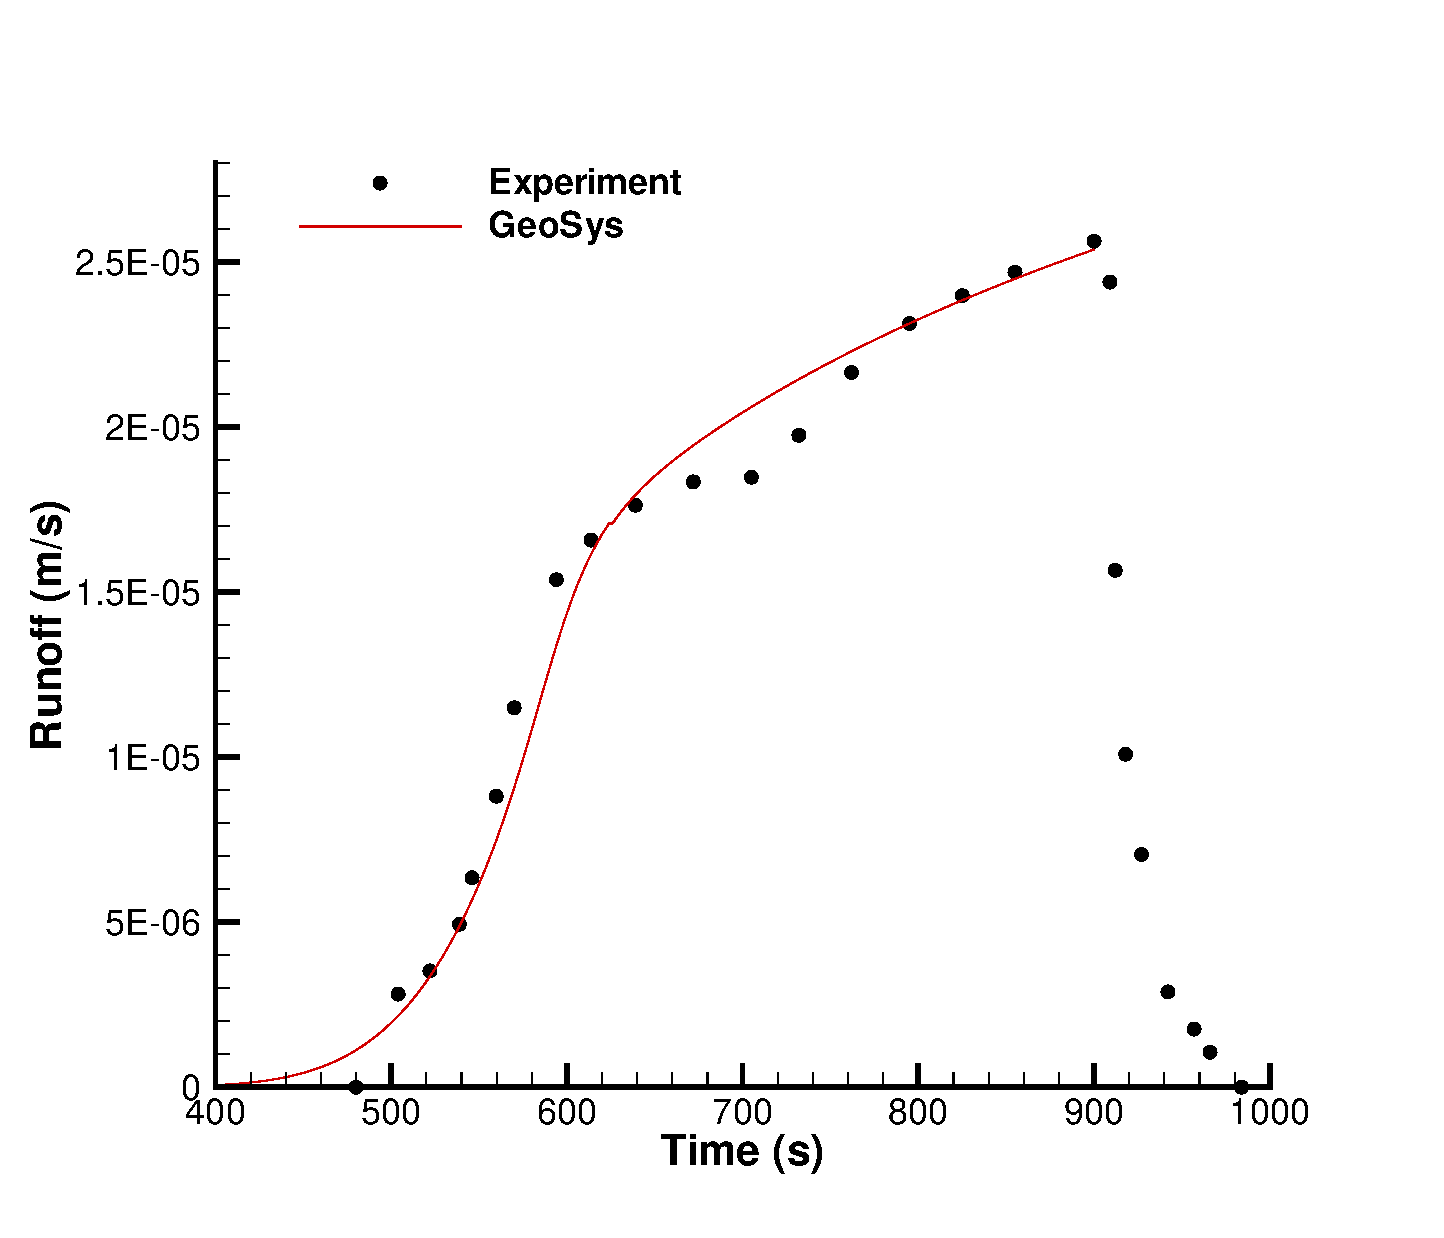
\includegraphics[width=0.75\columnwidth] {H_SFC/figures/Wool.eps}
 \caption{Measurements and simulation results by Geosys for the outflow hydrograph in the Horton overland flow example}
 \label{SFC:resultsWool}
\end{figure}
%
\subsubsection*{Benchmark deposit}
\begin{tabular}{|l|l|l|}
  \hline
  Benchmark & Problem type & Path in benchmark deposit \\
  \hline
  \emph{Wool\_quad} & H & benchmarks\verb \OVERLAND_FLOW\ \\
 \hline
\end{tabular}

